% Diagrama general de la metodología (Figura de la introducción del Capítulo 3).
% Compilar:  pdflatex diagrama_metodologia.tex   ->  diagrama_metodologia.pdf
\documentclass[border=3pt]{standalone}
\usepackage[utf8]{inputenc}
\usepackage[T1]{fontenc}
\usepackage{times}
\usepackage{amsmath}
\usepackage{tikz}
\usetikzlibrary{positioning, shapes.geometric, arrows.meta, fit, backgrounds, calc}

\begin{document}
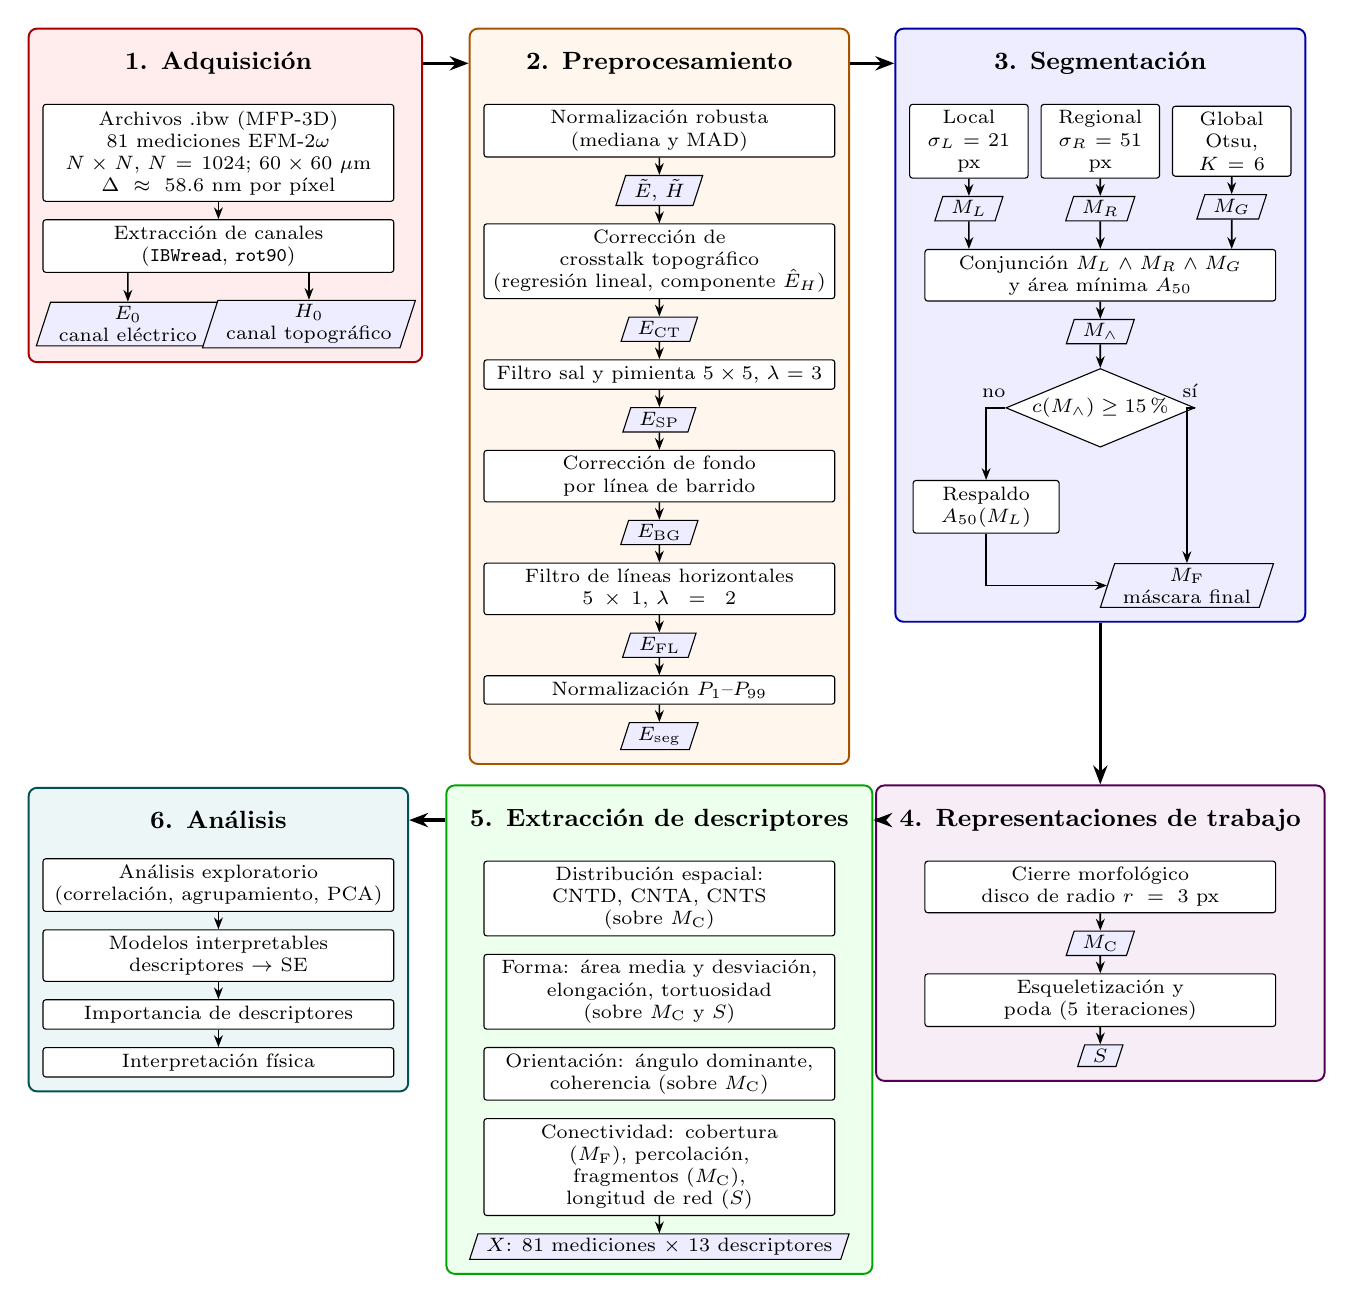
\begin{tikzpicture}[
    node distance = 0.22cm and 0.2cm,
    op/.style    = {draw, rectangle, rounded corners=1pt, fill=white, align=center,
                    font=\scriptsize, text width=#1, inner sep=2.2pt,
                    execute at begin node={\hyphenpenalty=10000\exhyphenpenalty=10000}},
    op/.default  = 4.3cm,
    var/.style   = {draw, trapezium, trapezium left angle=72, trapezium right angle=108,
                    trapezium stretches body, fill=blue!7, font=\scriptsize, align=center,
                    inner xsep=3pt, inner ysep=1.5pt},
    dec/.style   = {draw, diamond, aspect=2.4, fill=white, font=\scriptsize, inner sep=0.3pt, align=center},
    flow/.style  = {-{Stealth[length=1.5mm]}, semithick},
    big/.style   = {-{Stealth[length=2.4mm]}, very thick},
    title/.style = {font=\small\bfseries, align=center},
    stage/.style = {draw=#1!65!black, fill=#1!7, rounded corners=3pt, inner sep=5pt, line width=0.7pt}
]

% =====================================================================
% Fila superior: 1. Adquisición -> 2. Preprocesamiento -> 3. Segmentación
% =====================================================================

% ---- 1. Adquisición --------------------------------------------------
\node[title] (t1) at (0,0) {1. Adquisición};
\node[op] (a1) [below=0.25cm of t1] {Archivos .ibw (MFP-3D)\\81 mediciones EFM-2$\omega$\\$N\times N$, $N=1024$; $60\times60~\mu$m\\$\Delta \approx 58.6$~nm por píxel};
\node[op] (a2) [below=of a1] {Extracción de canales\\(\texttt{IBWread}, \texttt{rot90})};
\node[var] (a3) at ($(a2.south)+(-1.15,-0.65)$) {$E_0$\\canal eléctrico};
\node[var] (a4) at ($(a2.south)+(1.15,-0.65)$) {$H_0$\\canal topográfico};
\draw[flow] (a1) -- (a2);
\draw[flow] (a2.south -| a3) -- (a3);
\draw[flow] (a2.south -| a4) -- (a4);

% ---- 2. Preprocesamiento --------------------------------------------
\node[title] (t2) at (5.6,0) {2. Preprocesamiento};
\node[op] (b0) [below=0.25cm of t2] {Normalización robusta (mediana y MAD)};
\node[var] (v0) [below=of b0] {$\tilde E$, $\tilde H$};
\node[op] (b1) [below=of v0] {Corrección de crosstalk topográfico\\(regresión lineal, componente $\hat E_H$)};
\node[var] (v1) [below=of b1] {$E_{\mathrm{CT}}$};
\node[op] (b2) [below=of v1] {Filtro sal y pimienta $5\times5$, $\lambda=3$};
\node[var] (v2) [below=of b2] {$E_{\mathrm{SP}}$};
\node[op] (b3) [below=of v2] {Corrección de fondo por línea de barrido};
\node[var] (v3) [below=of b3] {$E_{\mathrm{BG}}$};
\node[op] (b4) [below=of v3] {Filtro de líneas horizontales $5\times1$, $\lambda=2$};
\node[var] (v4) [below=of b4] {$E_{\mathrm{FL}}$};
\node[op] (b5) [below=of v4] {Normalización $P_1$--$P_{99}$};
\node[var] (v5) [below=of b5] {$E_{\mathrm{seg}}$};
\foreach \x/\y in {b0/v0, v0/b1, b1/v1, v1/b2, b2/v2, v2/b3, b3/v3, v3/b4, b4/v4, v4/b5, b5/v5}
    \draw[flow] (\x) -- (\y);

% ---- 3. Segmentación -------------------------------------------------
\node[title] (t3) at (11.2,0) {3. Segmentación};
\node[op=1.35cm] (c2) [below=0.25cm of t3] {Regional\\$\sigma_R=51$ px};
\node[op=1.35cm] (c1) [left=0.15cm of c2] {Local\\$\sigma_L=21$ px};
\node[op=1.35cm] (c3) [right=0.15cm of c2] {Global\\Otsu, $K=6$};
\node[var] (m1) [below=of c1] {$M_L$};
\node[var] (m2) [below=of c2] {$M_R$};
\node[var] (m3) [below=of c3] {$M_G$};
\node[op] (c4) [below=0.35cm of m2] {Conjunción $M_L\wedge M_R\wedge M_G$\\y área mínima $A_{50}$};
\node[var] (m4) [below=of c4] {$M_\wedge$};
\node[dec] (d1) [below=0.3cm of m4] {$c(M_\wedge)\ge 15\,\%$};
\node[op=1.7cm] (c5) at ($(d1.south)+(-1.45,-0.75)$) {Respaldo\\$A_{50}(M_L)$};
\node[var] (m5) at ($(d1.south)+(1.1,-1.75)$) {$M_{\mathrm{F}}$\\máscara final};
\foreach \x/\y in {c1/m1, c2/m2, c3/m3, c4/m4, m4/d1}
    \draw[flow] (\x) -- (\y);
\foreach \m in {m1, m2, m3}
    \draw[flow] (\m) -- (\m |- c4.north);
\draw[flow] (d1.west) -| node[pos=0.3, above, font=\scriptsize] {no} (c5.north);
\draw[flow] (d1.east) -| node[pos=0.3, above, font=\scriptsize] {sí} (m5.north);
\draw[flow] (c5.south) |- (m5.west);

% ---- Recuadros de la fila superior ----------------------------------
\begin{scope}[on background layer]
\node[stage=red,    fit=(t1)(a1)(a2)(a3)(a4)] (s1) {};
\node[stage=orange, fit=(t2)(b0)(v5)] (s2) {};
\node[stage=blue,   fit=(t3)(c1)(c3)(c5)(m5)(d1)] (s3) {};
\end{scope}

% =====================================================================
% Fila inferior (de derecha a izquierda): 4 -> 5 -> 6
% =====================================================================
\coordinate (r2) at ($(s2.south)+(0,-0.7)$);

% ---- 4. Representaciones de trabajo ---------------------------------
\node[title] (t4) at (t3 |- r2) {4. Representaciones de trabajo};
\node[op] (e1) [below=0.25cm of t4] {Cierre morfológico\\disco de radio $r=3$ px};
\node[var] (w1) [below=of e1] {$M_{\mathrm{C}}$};
\node[op] (e2) [below=of w1] {Esqueletización y poda (5 iteraciones)};
\node[var] (w2) [below=of e2] {$S$};
\draw[flow] (e1) -- (w1);  \draw[flow] (w1) -- (e2);  \draw[flow] (e2) -- (w2);

% ---- 5. Extracción de descriptores ----------------------------------
\node[title] (t5) at (t2 |- r2) {5. Extracción de descriptores};
\node[op] (f1) [below=0.25cm of t5] {Distribución espacial: CNTD, CNTA, CNTS\\(sobre $M_{\mathrm{C}}$)};
\node[op] (f2) [below=of f1] {Forma: área media y desviación,\\elongación, tortuosidad (sobre $M_{\mathrm{C}}$ y $S$)};
\node[op] (f3) [below=of f2] {Orientación: ángulo dominante,\\coherencia (sobre $M_{\mathrm{C}}$)};
\node[op] (f4) [below=of f3] {Conectividad: cobertura ($M_{\mathrm{F}}$), percolación,\\fragmentos ($M_{\mathrm{C}}$), longitud de red ($S$)};
\node[var] (w3) [below=of f4] {$X$: 81 mediciones $\times$ 13 descriptores};
\draw[flow] (f4) -- (w3);

% ---- 6. Análisis -----------------------------------------------------
\node[title] (t6) at (t1 |- r2) {6. Análisis};
\node[op] (g1) [below=0.25cm of t6] {Análisis exploratorio\\(correlación, agrupamiento, PCA)};
\node[op] (g2) [below=of g1] {Modelos interpretables\\descriptores $\rightarrow$ SE};
\node[op] (g3) [below=of g2] {Importancia de descriptores};
\node[op] (g4) [below=of g3] {Interpretación física};
\draw[flow] (g1) -- (g2);  \draw[flow] (g2) -- (g3);  \draw[flow] (g3) -- (g4);

\begin{scope}[on background layer]
\node[stage=violet, fit=(t4)(e1)(w2)] (s4) {};
\node[stage=green,  fit=(t5)(f1)(w3)] (s5) {};
\node[stage=teal,   fit=(t6)(g1)(g4)] (s6) {};
\end{scope}

% =====================================================================
% Flujo entre etapas
% =====================================================================
\draw[big] (s1.east |- t1) -- (s2.west |- t1);
\draw[big] (s2.east |- t2) -- (s3.west |- t2);
\draw[big] (s3.south) -- (s4.north);
\draw[big] (s4.west |- t4) -- (s5.east |- t4);
\draw[big] (s5.west |- t5) -- (s6.east |- t5);
\end{tikzpicture}
\end{document}
